\chapter{$d(K^-, p)"\pi^-\Lambda"/"\pi^-\Sigma^0"$ mode}
\begin{figure}[htbp]
  \centering
  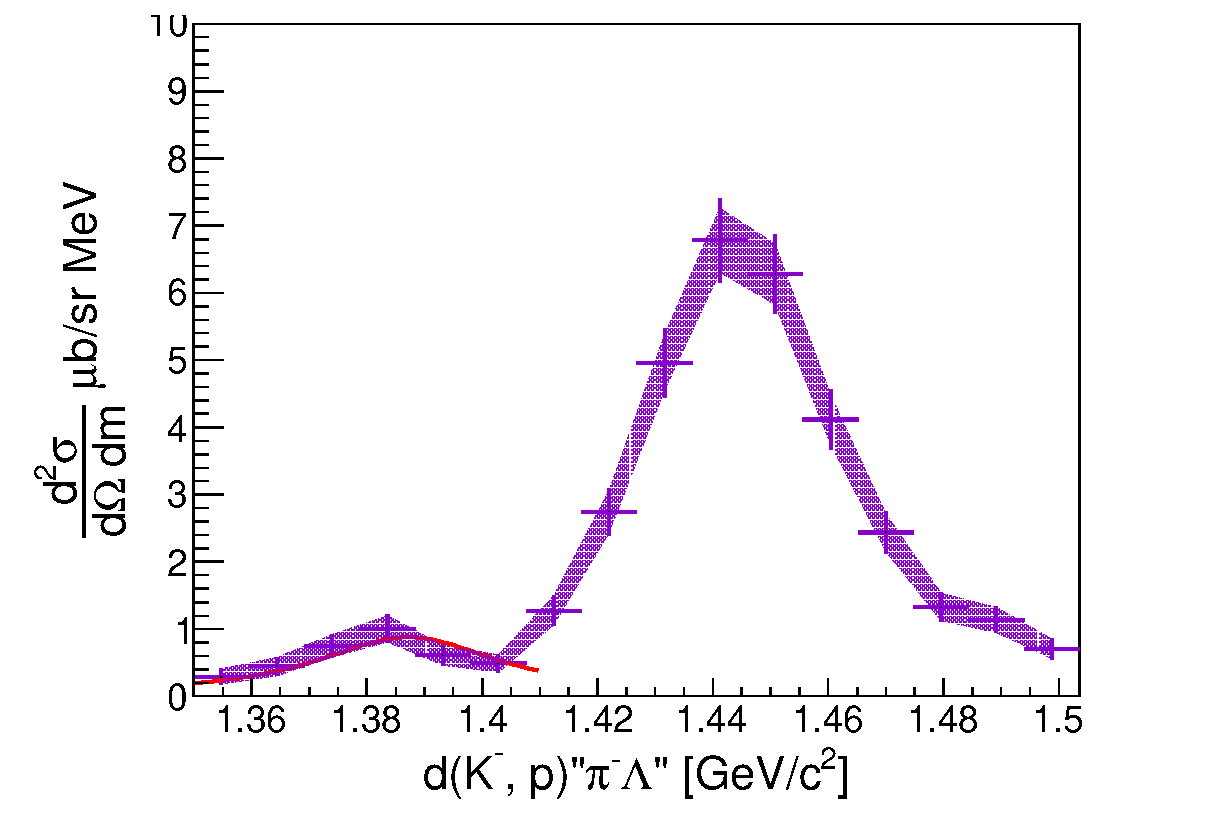
\includegraphics[width=10cm]{../pic/Dron/pimL_CS_wS1385.eps}
  \caption{
    This figure shows the obtained $d(K^-, p)"\pi^-\Lambda"$ spectrum with $\Sigma(1385)^-$ fitting which indicats as red line.
  }
  \label{fig:pimL_CS_appendix}
\end{figure}

\begin{figure}[htbp]
  \centering
  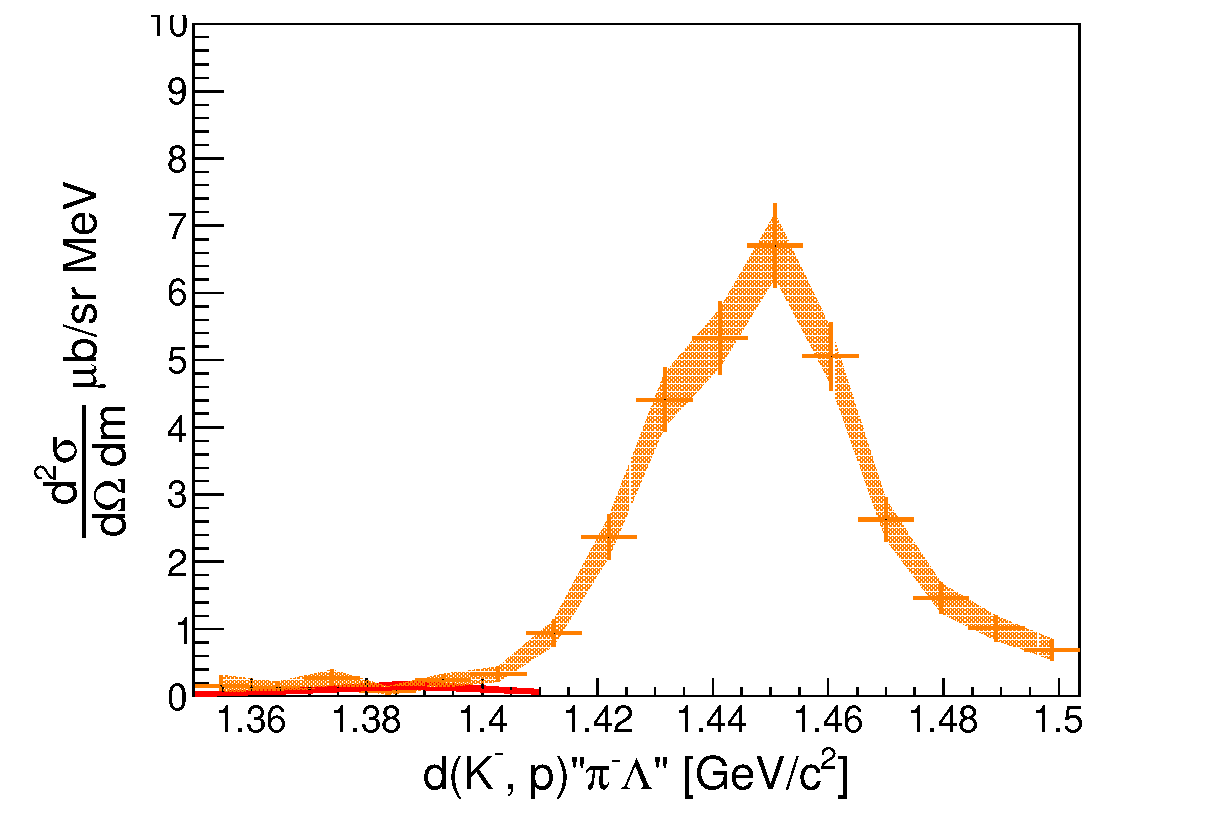
\includegraphics[width=10cm]{../pic/Dron/pimS0_CS_wS1385.eps}
  \caption{
    This figure shows the obtained $d(K^-, p)"\pi^- \Sigma^0"$ spectrum with $\Sigma(1385)^-$ contribution that was estimated from $\pi^- \Lambda$ mode.
  }
  \label{fig:pimS0_CS_appendix}
\end{figure}
We obtaine the cross section of the $d(K^-, p)"\pi^-\Lambda"$ that is observed some structure around the $\Sigma(1385)$ region as shown in Fig\ref{fig:pimL_CS_appendix}.
Although the $\Sigma(1305)$ whose isospin, spin and parity are $I(J^p)=1(3/2^+)$ is P-wave,
the pole due to the $\Sigma(1385)$ should appear 2-step effect that is constructive or destructive interferance term.
A constructive contribution is clearly observed in the spectrum that was fitted with fixd mass and width whose values were adopted at $1387.2MeV/c^2$ and $39.4MeV/c^2$ respectively that is PDG\cite{PDG} value.

The $\Sigma(1385)$ of the branching ratio of $\pi^-\Sigma^0$ against $\pi^-\Sigma^0$ is 0.135.
The contribution to $\pi^-\Sigma^0$ mode of this branging ratio was ploted with our obtained spectrum in Fig\ref{fig:pimS0_CS_appendix} that is almost consistent.

